\documentclass[border=6pt]{standalone}
\usepackage{tikz}
\begin{document}
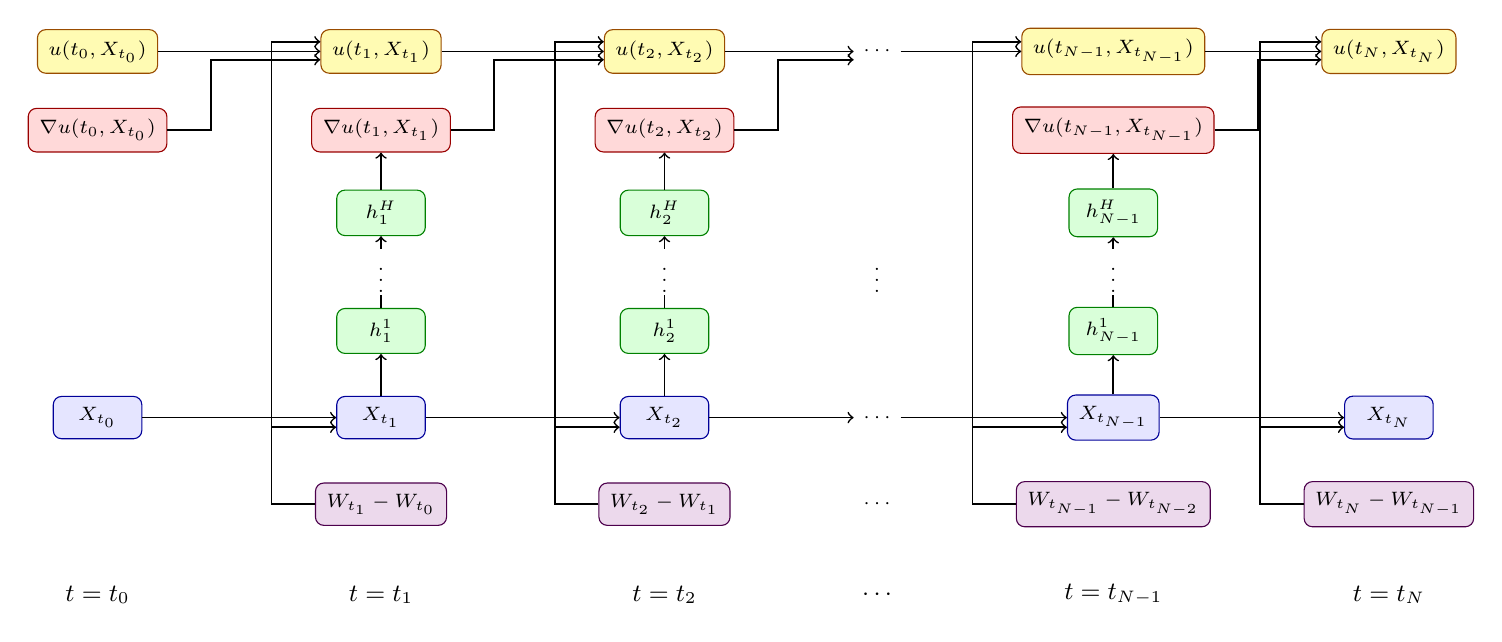
\begin{tikzpicture}[
  every node/.style={font=\scriptsize},
  un/.style={draw=orange!60!black, fill=yellow!30, rounded corners=3pt, inner sep=4pt},
  gn/.style={draw=red!60!black, fill=red!15, rounded corners=3pt, inner sep=4pt},
  hn/.style={draw=green!50!black, fill=green!15, rounded corners=3pt, inner sep=4pt, minimum width=3.2em},
  xn/.style={draw=blue!60!black, fill=blue!10, rounded corners=3pt, inner sep=4pt, minimum width=3.2em},
  wn/.style={draw=violet!60!black, fill=violet!15, rounded corners=3pt, inner sep=4pt},
  ar/.style={->, semithick}]

% ---------------- column t0 ----------------
\node[un] (u0) at (0, 5.4) {$u(t_0, X_{t_0})$};
\node[gn] (g0) at (0, 4.4) {$\nabla u(t_0, X_{t_0})$};
\node[xn] (x0) at (0, 0.75) {$X_{t_0}$};
\node at (0, -1.5) {\small $t = t_0$};

% ---------------- column t1 ----------------
\node[un] (u1) at (3.6, 5.4) {$u(t_1, X_{t_1})$};
\node[gn] (g1) at (3.6, 4.4) {$\nabla u(t_1, X_{t_1})$};
\node[hn] (hH1) at (3.6, 3.35) {$h^{H}_{1}$};
\node[hn] (h11) at (3.6, 1.85) {$h^{1}_{1}$};
\node[xn] (x1) at (3.6, 0.75) {$X_{t_1}$};
\node[wn] (w1) at (3.6, -0.35) {$W_{t_1} - W_{t_0}$};
\node at (3.6, -1.5) {\small $t = t_1$};

% ---------------- column t2 ----------------
\node[un] (u2) at (7.2, 5.4) {$u(t_2, X_{t_2})$};
\node[gn] (g2) at (7.2, 4.4) {$\nabla u(t_2, X_{t_2})$};
\node[hn] (hH2) at (7.2, 3.35) {$h^{H}_{2}$};
\node[hn] (h12) at (7.2, 1.85) {$h^{1}_{2}$};
\node[xn] (x2) at (7.2, 0.75) {$X_{t_2}$};
\node[wn] (w2) at (7.2, -0.35) {$W_{t_2} - W_{t_1}$};
\node at (7.2, -1.5) {\small $t = t_2$};

% ---------------- dots column ----------------
\node (du) at (9.9, 5.4) {$\cdots$};
\node at (9.9, 2.6) {$\vdots$};
\node (dx) at (9.9, 0.75) {$\cdots$};
\node (dw) at (9.9, -0.35) {$\cdots$};
\node at (9.9, -1.5) {\small $\cdots$};

% ---------------- column t_{N-1} ----------------
\node[un] (u3) at (12.9, 5.4) {$u(t_{N-1}, X_{t_{N-1}})$};
\node[gn] (g3) at (12.9, 4.4) {$\nabla u(t_{N-1}, X_{t_{N-1}})$};
\node[hn] (hH3) at (12.9, 3.35) {$h^{H}_{N-1}$};
\node[hn] (h13) at (12.9, 1.85) {$h^{1}_{N-1}$};
\node[xn] (x3) at (12.9, 0.75) {$X_{t_{N-1}}$};
\node[wn] (w3) at (12.9, -0.35) {$W_{t_{N-1}} - W_{t_{N-2}}$};
\node at (12.9, -1.5) {\small $t = t_{N-1}$};

% ---------------- column t_N ----------------
\node[un] (u4) at (16.4, 5.4) {$u(t_N, X_{t_N})$};
\node[xn] (x4) at (16.4, 0.75) {$X_{t_N}$};
\node[wn] (w4) at (16.4, -0.35) {$W_{t_N} - W_{t_{N-1}}$};
\node at (16.4, -1.5) {\small $t = t_N$};

% ---------------- subnetworks (vertical chains) ----------------
\foreach \c in {1,2,3}{
  \draw[ar] (x\c) -- (h1\c);
  \draw[ar] (h1\c) -- (hH\c);
  \draw[ar] (hH\c) -- (g\c);
}
\node[fill=white, inner sep=1pt] at (3.6, 2.6) {$\vdots$};
\node[fill=white, inner sep=1pt] at (7.2, 2.6) {$\vdots$};
\node[fill=white, inner sep=1pt] at (12.9, 2.6) {$\vdots$};

% ---------------- u chain ----------------
\draw[ar] (u0) -- (u1);
\draw[ar] (u1) -- (u2);
\draw[ar] (u2) -- (du);
\draw[ar] (du) -- (u3);
\draw[ar] (u3) -- (u4);

% ---------------- X chain ----------------
\draw[ar] (x0) -- (x1);
\draw[ar] (x1) -- (x2);
\draw[ar] (x2) -- (dx);
\draw[ar] (dx) -- (x3);
\draw[ar] (x3) -- (x4);

% ---------------- gradient feeds into the next u ----------------
\draw[ar] (g0.east) -- ++(0.55,0) |- ([yshift=-3pt]u1.west);
\draw[ar] (g1.east) -- ++(0.55,0) |- ([yshift=-3pt]u2.west);
\draw[ar] (g2.east) -- ++(0.55,0) |- ([yshift=-3pt]du.west);
\draw[ar] (g3.east) -- ++(0.55,0) |- ([yshift=-3pt]u4.west);

% ---------------- Brownian increments feed X and u ----------------
\foreach \c in {1,2,3,4}{
  \draw[ar] (w\c.west) -- ++(-0.55,0) |- ([yshift=-3.5pt]x\c.west);
  \draw[ar] (w\c.west) -- ++(-0.55,0) |- ([yshift=3.5pt]u\c.west);
}
\end{tikzpicture}
\end{document}
